% !TeX root = ../main.tex
\documentclass[./../main.tex]{subfiles}

\begin{document}
\section{Đặt vấn đề}
Hiện nay, phương thức tấn công phổ biến nhất đối với các tệp PDF độc hại bắt nguồn từ việc nhúng các đoạn mã javascript - những đoạn mã mà sẽ được thực thi bởi ứng dụng đọc tệp PDF. Lợi dụng nhiều lỗ hổng bảo mật nghiêm trọng từ các trình đọc PDF, có thể kể đến nhiều nhất là Acrobat Reader, các kẻ tấn công đã sử dụng mã javascript để thực hiện khai thác các lỗ hổng đó, nhằm xâm nhập vào hệ thống máy tính nạn nhân và thực hiện những hành vi độc hại. Việc phân tích tĩnh và trích xuất các đặc trưng thực hiện ở chương 2 chỉ mang tính chất thống kê và kiểm tra sự tồn tại của javascript, chưa thực sự đi sâu vào khai thác các hành vi của mã. Bên cạnh đó, với sự phát triển của kỹ thuật làm rối, các đoạn mã javascript càng trở nên khó phát hiện hơn, hoặc được xây dựng trông như một đoạn mã lành tính, gây nhiễu cho các mô hình phân loại học máy. Có thể thấy các đặc trưng đã trích xuất chưa thực sự đem lại một kết quả tốt với các mã có nhúng javascript.
Ở chương này, tôi đề xuất một phương pháp gồm hai giai đoạn để xử lý các tệp PDF có chứa javascript.
\begin{itemize}
	\item Giai đoạn một thực hiện trích xuất đặc trưng cơ bản và đưa qua bộ phân loại Zero False Positive với mục tiêu của giai đoạn này là tạo nên một tường lửa nhạy bén với các tệp độc, đảm bảo loại bỏ được những tệp chắc chắn là độc, tức mô hình học máy không gây ra dương sai (FP).
	\item Giai đoạn hai được đề xuất sẽ xử lý các tệp PDF được gán nhãn sạch, bằng các kỹ thuật xử lý nâng cao, đòi hỏi thời gian và chi phí phân tích hơn để tìm ra chính xác tệp PDF độc hại nào còn sót lại.
\end{itemize}

\section{Bộ phân loại Zero False Positive}
Bộ phân loại Zero False Positive được đề xuất trong giai đoạn một để mang tới một kết quả phân loại không có gán nhãn dương sai. Ý tưởng xây dựng dựa trên mô hình được đề xuất trong công bố của Mohammad Sayad Haghighi và cộng sự \cite{zfp}.

\subsection{Thuật toán phân loại lặp với mục tiêu FP = 0}
% figure
\begin{figure}[ht!]
	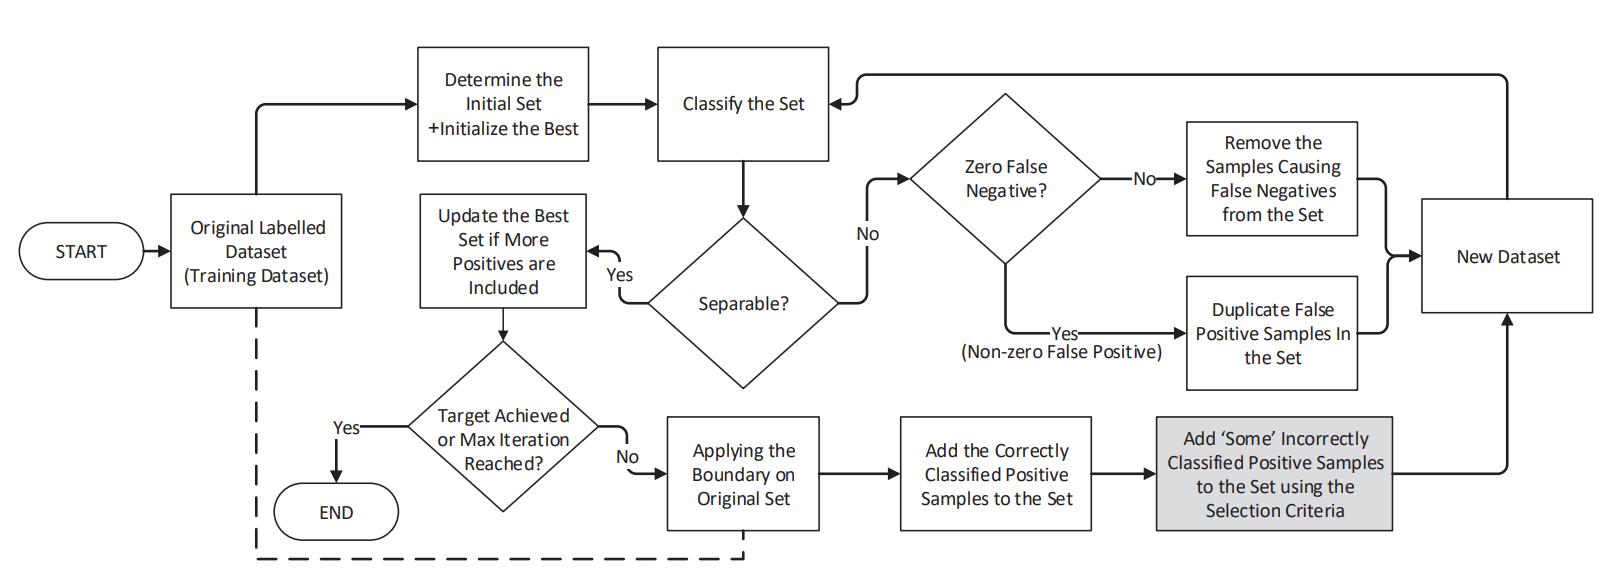
\includegraphics[width=\linewidth]{./images/zfp_flow_chart.png}
	\caption{Sơ đồ luồng hoạt động của thuật toán lặp Zero False Positive}
	\label{fig:zfp_flow_chart}
\end{figure}

% figure
\begin{figure}[ht!]
	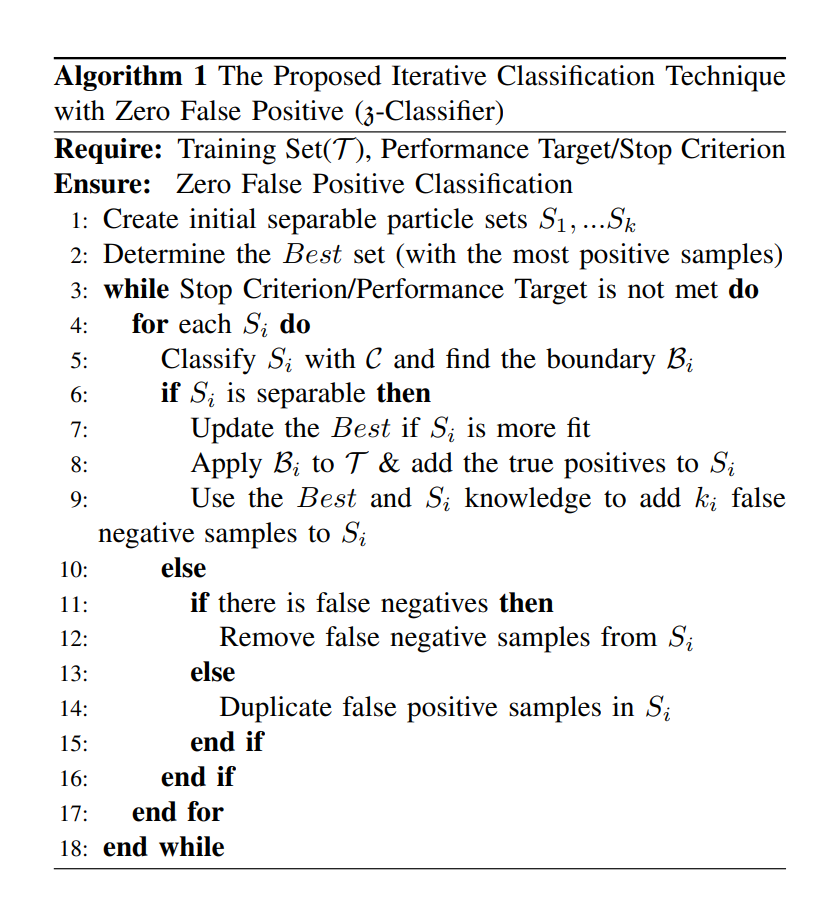
\includegraphics[width=\linewidth]{./images/algorithm_zfp.png}
	\caption{Mã giả thuật toán lặp Zero False Positive}
	\label{fig:algorithm}
\end{figure}

\subsection{Thực nghiệm và đánh giá kết quả}
Tiến hành thực nghiệm để kiểm định mô hình trên tập huấn luyện gồm các tệp PDF đã được trích xuất đặc trưng thống kê và đặc trưng cấu trúc trong chương 2. Kết quả cho thấy số lượng FP qua các vòng lặp đều được đảm bảo bằng 0 và số lượng FN giảm dần. Tuy nhiên, từ vòng lặp thứ 700 - 1000, kết quả FN không giảm, duy trì số lượng 97, với tỉ lệ FNR bằng 0.0095.

\begin{table}[]
	\centering
	\caption{Kết quả của thuật toán phân loại Zero False Positive trên tập dữ liệu đã trích xuất}
	\label{tab:ket_qua_thuat_toan_phan_loai}
	\begin{tabular}{|c|c|c|c|c|}
		\hline
		\textbf{Iteration} & \textbf{TN} & \textbf{FP} & \textbf{FN} & \textbf{TP} \\ \hline
		0                  & 7423        & 0           & 2993        & 7220        \\ \hline
		5                  & 7423        & 0           & 361         & 9852        \\ \hline
		10                 & 7423        & 0           & 255         & 9988        \\ \hline
		50                 & 7423        & 0           & 133         & 10080       \\ \hline
		100                & 7423        & 0           & 107         & 10106       \\ \hline
		200                & 7423        & 0           & 105         & 10108       \\ \hline
		500                & 7423        & 0           & 100         & 10113       \\ \hline
		700                & 7423        & 0           & 97          & 10116       \\ \hline
		1000               & 7423        & 0           & 97          & 10116       \\ \hline
	\end{tabular}
\end{table}

Ngoài ra, mô hình được tiến hành thử nghiệm trên một số tập dữ liệu khác. Bộ dữ liệu đặc trưng tệp PDF được trích xuất và công bố bởi đội ngũ phát triển Hidost [ref hidost reputation] với một số lượng lớn các mẫu PDF độc hại được thu thập qua nhiều năm. Tôi đã liên hệ Nedim Srndic, một trong những tác giả của Hidost để xin phép sử dụng bộ dữ liệu đặc trưng trong phạm vi khóa luận này. Bộ dữ liệu được phân thành nhiều tập, và dưới đây là kết quả của hai tập dữ liệu khi thử nghiệm trên mô hình phân loại Zero False Positive.

\begin{table}[]
	\centering
	\caption{Kết quả thuật toán phân loại Zero False Positive trên tập dữ liệu Hidost (1)}
	\label{tab:ket_qua_thuat_toan_phan_loai_hidost}
	\begin{tabular}{|c|c|c|c|c|}
		\hline
		\textbf{Iteration} & \textbf{TN} & \textbf{FP} & \textbf{FN} & \textbf{TP} \\ \hline
		0                  & 142796      & 0           & 1851        & 4406        \\ \hline
		10                 & 142796      & 0           & 410         & 5847        \\ \hline
		50                 & 142796      & 0           & 287         & 5970        \\ \hline
		100                & 142796      & 0           & 272         & 5985        \\ \hline
		120                & 142796      & 0           & 271         & 5986        \\ \hline
		160                & 142796      & 0           & 271         & 5986        \\ \hline
	\end{tabular}
\end{table}

\begin{table}[]
	\centering
	\caption{Kết quả thuật toán phân loại Zero False Positive trên tập dữ liệu Hidost (2)}
	\label{tab:ket_qua_thuat_toan_phan_loai_hidost_2}
	\begin{tabular}{|c|c|c|c|c|}
		\hline
		\textbf{iteration} & \textbf{TN} & \textbf{FP} & \textbf{FN} & \textbf{TP} \\ \hline
		0                  & 132465      & 0           & 4919        & 2484        \\ \hline
		10                 & 132465      & 0           & 539         & 6864        \\ \hline
		50                 & 132465      & 0           & 317         & 7086        \\ \hline
		100                & 132465      & 0           & 305         & 7098        \\ \hline
		190                & 132465      & 0           & 305         & 7098        \\ \hline
	\end{tabular}
\end{table}

Với số lượng tập sạch lớn, chênh lệch so với số lượng tập độc, tập dữ liệu của Hidost yêu cầu thời gian chạy lớn khi thực hiện thuật toán phân loại Zero False Positive, và tỉ lệ FNR còn khá cao, 0.043 với tập thứ 1 và 0.041 ở tập thứ 2.

\section{Phương hướng xử lý các tệp được gán nhãn sạch}
Sau khi lọc các tệp PDF có chứa mã javascript qua mô hình phân loại Zero False Positive, các tệp được gán nhãn sạch sẽ có nguy cơ chứa các tệp độc hại. Từ đây các mẫu này sẽ tiếp tục được xử lý tại giai đoạn hai: thực hiện phân tích và trích xuất những đặc trưng liên quan tới javascript được nhúng trong tài liệu PDF. Trong phần này, một số cách tiếp cận xử lý nâng cao bao gồm cả phân tích tĩnh và phân tích động sẽ được giới thiệu.
\end{document}

